

% Dies ist die Preambel
% \documentclass[12pt,a4paper,bibtotoc, twoside, cleardoublepage=empty]{article} % twoside
\documentclass[12pt,a4paper,bibtotoc, cleardoublepage=empty]{article}  % oneside centered
\bibliographystyle{plain}

\usepackage{pdfpages} % import pdf


% das ist Standard - nie ohne aus dem Haus gehen
\usepackage[german]{babel}
% Biber!!!!!!!!!!!!!!!!!!


\usepackage{ebgaramond}

\usepackage{typearea}
\usepackage[style=authortitle]{biblatex}
\usepackage[babel,german=guillemets]{csquotes}
\bibliography{lit/literatur}



\usepackage[onehalfspacing]{setspace}

\usepackage{tabularx} % in the preamble

% Fu�noten auch in �berschriften
\usepackage[stable]{footmisc}

% Bilder
\usepackage{graphicx}
\graphicspath{ {../img/} } 
\usepackage{float} 

% Seitenraender 
\usepackage{geometry}

%\geometry{a4paper, top=20mm, left=35mm, right=20mm, bottom=20mm,headsep=12mm, footskip=12mm} % twoside
\geometry{a4paper, top=20mm, left=20mm, right=20mm, bottom=20mm,headsep=12mm, footskip=12mm} % oneside centered


%\usepackage{natbib}


%Hinweisbox
\usepackage{calc}
\usepackage{hhline} 
\usepackage{multirow} 
\usepackage{xcolor}
\usepackage{colortbl}
\usepackage{graphicx}

\newlength{\iconwidth}
\setlength{\iconwidth}{1cm}

\definecolor{boxheadcol}{gray}{.6}
\definecolor{boxcol}{gray}{.9}

\newenvironment{displaybox}[2]{%
  \begin{center}
    \setlength\arrayrulewidth{0.75pt}%
    \arrayrulecolor{white}%
    \renewcommand{\arraystretch}{1.3}%
    \begin{tabular}{p{\iconwidth}p{\linewidth-4\tabcolsep-\iconwidth}}
      \multirow{2}{*}{#2}&\cellcolor{boxheadcol}\textbf{\sffamily\color{white}#1} \\%
      \hhline{~-}%
      &\cellcolor{boxcol}%
}{%
      \\
    \end{tabular}
  \end{center}%
}


\newenvironment{Tipp}{%
\begin{displaybox}{Tipp}{
\includegraphics[width=\iconwidth]{img/com/icon-tipp}}}%
{\end{displaybox}}

\newenvironment{Hinweis}{%
\begin{displaybox}{Hinweis}{
\includegraphics[width=\iconwidth]{img/com/icon-hinweis}}}%
{\end{displaybox}}
%Hinweisbox ende

% Standart Kopfzeile 
\pagestyle{headings}
  
% Referenzen

\usepackage{hyperref}
\hypersetup{
  colorlinks=true,
  linkcolor=black,
	citecolor=black,
  urlcolor=blue,
  pdfborder={0 0 0}
}

% Mit Mausklick zum Ziel
\usepackage{nameref}
% URLs
\usepackage{url} 



% Umlaute:
% Immer nur einen inputenc verwenden, sonst Fehler!
% Linux
% \usepackage[latin1]{inputenc} 
% Windows
\usepackage[utf8]{inputenc}

% Umlaute auch in der PDF
\usepackage[T1]{fontenc}

% Fuer jede Section eine neue Seite
\let\stdsection\section
\renewcommand\section{\newpage\stdsection}

% Fuer jede SubSection eine neue Seite
%\let\stdsubsection\subsection
%\renewcommand\subsection{\newpage\stdsubsection}

%\usepackage{natbib}	% Literaturverzeichnis

% \usepackage{skull}	% alles hat ein Ende

\usepackage{color}	% bring Farbe ins Spiel
% Fuer Codebeispiele
\definecolor{DarkPurple}{rgb}{0.4,0.1,0.4}
\definecolor{DarkCyan}{rgb}{0.0,0.5,0.4}
\definecolor{LightLime}{rgb}{0.4,0.6,0.5}
\definecolor{Blue}{rgb}{0.0,0.0,1.0}

\definecolor{forestgreen}{RGB}{34,139,34}
\definecolor{orangered}{RGB}{239,134,64}
\definecolor{darkblue}{rgb}{0.0,0.0,0.6}
\definecolor{gray}{rgb}{0.4,0.4,0.4}

% sch?nere Serifenfonts
\usepackage{times}		
\usepackage{lmodern}
	
% deutsche Abs?tze
\parskip2ex		% Absatzabsstand	
\parindent0ex		% Absatzeinzug

% keine Hurenkinder und Schusterjungen
\clubpenalty=10000
\widowpenalty=10000

% Fuer mehr Codeschnipsel Funktionen
\usepackage{moreverb}

\usepackage{listings}

% f?r Java-Bezeichner und -Keywords im Flie?text
\newcommand{\code}[1]{\small\lstinline[style=InlineJava]!#1!\normalsize}
%\newcommand{\code}[1]{\scriptsize\texttt{#1}\normalsize}

% fuer Listings mit Eintrag im Inhaltsverzeichnis
%\newcommand{\newlisting}[2]{
%\subsubsection*{Listing \ref{lst:#1}: #2}
%\addcontentsline{toc}{subsubsection}{\ref{lst:#1}. #2}}

\let\underscore\_
\newcommand{\myunderscore}{\renewcommand{\_}{\underscore\hspace{0pt}}}
%Issue the changed underscore command to the whole document.
\myunderscore

\lstdefinestyle{Java}
{
language=Java,
numberfirstline,
numberstyle=\tiny\sffamily,
tabsize=5,
captionpos=b,
aboveskip=1em,
belowskip=1em,
columns=flexible,
xleftmargin=2em,
xrightmargin=1em,
frame=single,
frameround=tttt,
commentstyle=\itshape\color{LightLime},
keywordstyle=\bfseries\color{DarkPurple},
basicstyle=\footnotesize\ttfamily,
stringstyle=\color{Blue},
showstringspaces=false,
}

\lstdefinestyle{XML} {
    language=XML,
    extendedchars=true, 
    breaklines=true,
    breakatwhitespace=true,
    emph={},
    emphstyle=\color{red},
    basicstyle=\ttfamily,
    columns=fullflexible,
    commentstyle=\color{gray}\upshape,
    morestring=[b]",
    morecomment=[s]{<?}{?>},
    morecomment=[s][\color{forestgreen}]{<!--}{-->},
    keywordstyle=\color{orangered},
    stringstyle=\ttfamily\color{black}\normalfont,
    tagstyle=\color{darkblue}\bf,
    morekeywords={attribute,xmlns,version,type,release},
}




\lstnewenvironment{javalisting}[1][]
{
	\lstset{language=Java, 
					 style=Java
	}
}
{}

\newenvironment{javalistingfigure}
{
\begin{figure}
\begin{javalisting}
}
{
\end{javalisting}
	\caption{asasas}
	\label{fig:javalisting}
\end{figure}
}


%\lstnewenvironment{javalisting}
%{
%\begin{center}
	%\begin{figure}

%		\begin{lstlisting}[style=Java]
		
		%		public class UserSession implements Serializable{}

%}
%{
%		\end{lstlisting} 

		%\caption{dsdsds}
		%\label{fig:sddsdsds}
		
	%\end{figure}
%\end{center}
%}

% Strikeout
\usepackage{ulem}

% Zeilenumbruch Bib
\renewcommand*{\labelnamepunct}{\newunitpunct\par}

\usepackage{chngcntr}
\counterwithin{figure}{section}

\begin{document}
 

%%% SIMPLE TITLE

%\frontmatter
\pagestyle{empty}
\clearpage

\newcommand*{\titleUL}{\begingroup% Hochschule Harz
\begin{center}

%\rule{\textwidth}{0.25pt}\par
% -- LOGO

\includegraphics[width=0.35\textwidth]{img/hsharz/logo.png}

\LARGE{\textsc{Bericht zur Wissensvermittlung zum Tutorium der Lehrveranstaltung Objektorientierte Programmierung}}
\vspace{0.8\baselineskip}

\vfill

%
\includegraphics[width=0.6\textwidth]{../img/cd/logo.jpg}

\vfill

\normalsize


\begin{tabular}{r c l}
Alexander Johr & u34584 & m27007 \\
\hline
Prüfer: &  Prof. Daniel Ackermann & \\
\end{tabular}

  

%
\includegraphics{../img/hsharz/logo.png}




\vfill

Wernigerode, D-38855

\large 
31. August 2019

\end{center}

\endgroup}

% invoke defined title-command
\titleUL

%\includepdf[pages={1}]{FilmanalyseLolarenntDeckblatt.pdf}
 

\thispagestyle{plain}
\pagestyle{plain}

\tableofcontents

\listoffigures
 

\section{Report}

Die Wissensvermittlung im Tutorium für die Lehrveranstaltung Objektorientierte Programmierung verlief äußerst gut. Über das Semester kamen immer mehr und mehr Studenten in mein Tutorium. Auch Studierende, die ursprünglich einem anderen Tutor zugeteilt wurden, sahen sich mein Tutorium an und blieben dann bei mir (Abb. \ref{fig:Tutoriumsraum}).

\begin{figure}[htbp]
	\centering
		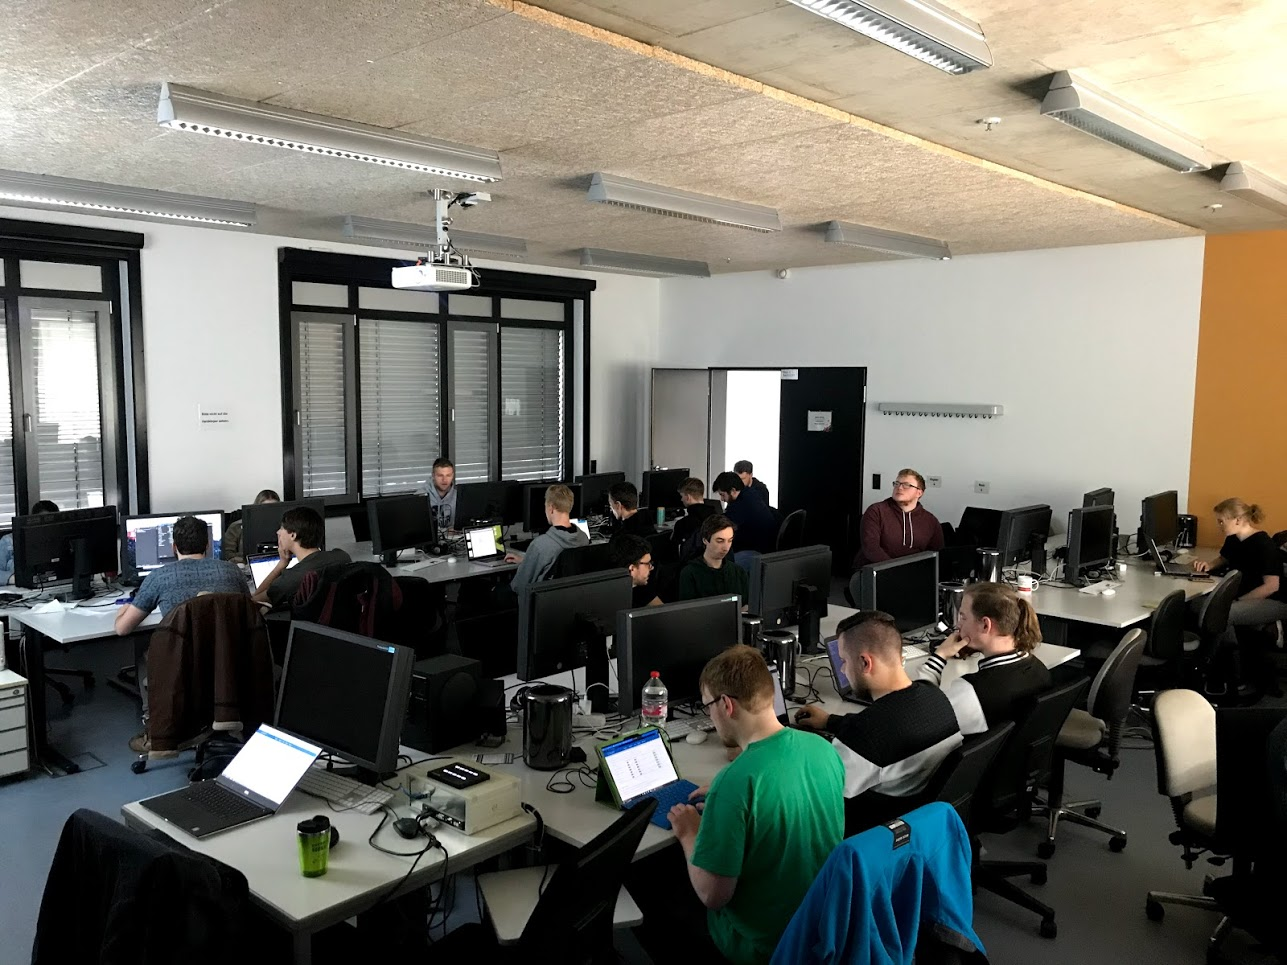
\includegraphics[width=1.00\textwidth]{img/Tutorium.jpg}
	\caption[Von interessierten Studierenden gefüllter Tutoriumsraum]{Von interessierten Studierenden gefüllter Tutoriumsraum}
	\label{fig:Tutoriumsraum}
\end{figure}

\subsection{Feedback der Studierenden}

Nach dem Tutorium holte ich mir Feedback von den Studierenden ein. Einige fanden das Tutorium so gut, dass sie sich wünschten, dass ich für sie noch mal einer Prüfungsvorbereitung anbiete. Bei Befragungen gaben die Studierenden an, dass sie das Tutorium für sehr gut befunden haben. Ich frage die Studierenden auch, ob aus ihrer Sicht noch Verbesserungspotenzial besteht. Die Studierenden waren der Meinung, dass es so, wie ich den Stoff anbiete, perfekt sein und ihnen keine Idee kämen, wie ich das Tutorium noch besser leiten könnte. Auch wenn mir diese Meinung schmeichelt, weiß ich um ein paar Punkte, die ich in Zukunft noch verbessern möchte.

In fast jedem Tutorium demonstrierte ich die Algorithmen, indem ich sie im Debugger vorführte. Ich zeigte den Studierenden den Umgang mit dem Debugger und setzte einige Mal sogar voraus, dass mir die Studierenden die Ergebnisse im Debugger zeigen. Erst wenn alle Studierenden den gleichen Wert in der Ausgabe demonstrieren konnten, kümmerten wir uns um die nächste Aufgabe. Die Studierenden gaben an, dass sie das als sehr positiv empfanden und sie mit dem Debugger im vorigen Semester wenig bis gar keine Erfahrung sammelten. Sie berichteten, nun das Gefühl zu haben, über den Debugger mehr Verständnis über den von ihnen geschriebenen Programmcode zu erlangen.

\subsection{Vorgehen}


Ich habe mir vor fast jedem Tutorium die Übungsaufgabe angesehen, welche die Studenten in dieser Woche bearbeiten müssen. Dann überlegte ich mir ein Minimalbeispiel, welches man in dem Tutorium schaffen kann.

Ich überlege mir die Übung aus mehreren Gründen:

Zum einen war es notwendig, sich die Aufgabe vorher anzusehen, um abzuschätzen, welche Grundlagen die Studenten für diese Aufgabe benötigen und welche die höchste Priorität haben.

Zum anderen, um sicher zu sein, dass während des Tutoriums keine Schwierigkeiten auftreten. Dafür programmiere ich die Übung zuvor selbst und überprüfe sie auf Lauffähigkeit und korrekte Ausgabe. Würde ich das nicht tun, ist die Wahrscheinlichkeit sehr groß, dass ich im Tutorium Fehler im eigenen Quellcode oder in meiner Entwicklungsumgebung finden muss. Aus privaten Gründen war ich einmal nicht in der Lage, die Übung vorzubereiten. Dann wurde mir auch klar, wie sinnvoll es war, die Übungen immer vorher zu testen. Denn während ich in dem Tutorium die Lösung für das Problem überlegte und die Studierenden mit mir gemeinsam entwickelten, fielen logische Fehler auf. Dadurch war es notwendig, Quellcode aus bereits geschriebenen Dateien zu modifizieren. Die Studierenden mussten das ebenso tun. Das führte zu Missverständnissen und unterschiedlichen, miteinander inkompatiblen, Versionen der Dateien. Für einige Studierenden war dann eine individuelle Betreuung notwendig, sodass ihr Quellcode wieder lauffähig war.

Dass alle Studierenden mitkommen, war mir auch besonders wichtig. Ich wollte, dass zu jedem Zeitpunkt alle Studierenden mitarbeiten können und niemand das Gefühl hat, abgehängt zu sein, da er nicht die nötige Erfahrung mitbringt. Daher fügte ich in regelmäßigen Abständen Momente ein, in denen ich mir die Ergebnisse aller Studierenden ansah. Gab es auch nur bei einem studierenden Schwierigkeiten, die ihm das Weiterarbeiten behinderten, so lösten wir das Problem gemeinsam.

Einige Male befürchtete ich, dass das von den Studierenden im Minimalbeispiel gelernte Wissen nicht ausreichen könnte. Daher habe ich im Anschluss an das Tutorium angeboten, dass die Studierenden in einem weiteren Unterrichtsblock noch mehr Details erfahren können. Dies wurde vom größten Teil der Studierenden angenommen. Lediglich Studierende, die terminlich gebunden waren, verließen das Tutorium.

\subsection{Fazit und Ausblick}

Ich programmierte alle Übungen mit den Studenten gemeinsam. Das von mir überlegte Minimalbeispiel konnten wir in fast allen Tutoriums Blöcken vollenden. Ich bin mir jedoch deutlich darüber im Klaren, dass diese Lernmethode einen Nachteil hat. Wenn ich Studierenden mit mir gemeinsam entwickeln, haben sie dabei die Möglichkeit, den aktuellen Code abzuschreiben, ohne darüber weiter nachzudenken. Dann lernen die Studierenden das Programmieren nicht, sie üben lediglich das Abschreiben von Code.
Daher bezog ich das Publikum häufig mit ein, indem ich fragte, welchen Schritt wir wohl als Nächstes angehen sollten. Ich ließ mir dann von den Studierenden diktieren, was ich als Nächstes eingeben muss. 

Mein Wunsch war es aber darüber hinaus, die Studenten häufiger Programmteile ganz selbstständig zu schreiben zu lassen. Durch die hohe Menge an Themen, die die Studenten bereits in diesem Semester lernen müssen, war mir das leider nicht möglich. 
Ich habe allerdings von Zeit zu Zeit die Studierenden gebeten, die letzte Teile des Quellcodes selbst zu schreiben und damit den Algorithmus zu vollenden.
 
Ein Großteil der Studenten schaffte das nicht, was mir zeigt, dass sie wohl schon im ersten Semester beim Erlernen der Grundlagen Schwierigkeiten hatten, hinterherzukommen. Fähigkeiten, die ich in meinem Tutorium lehrte und regelmäßig wiederholte, stellten für die Studierenden dagegen keine Schwierigkeiten dar. Daher wurde mein Wunsch umso größer, das Tutorium für Programmierung 1 im nächsten Semester zu übernehmen. So kann ich den gleichen Übungsstil auch bei den Grundlagen der Programmierung anwenden.

\end{document}